\documentclass[12pt, oneside]{article} 
\usepackage{amsmath, amsthm, amssymb, calrsfs, wasysym, verbatim, bbm, color,
graphics, geometry}
\usepackage[dvipsnames]{xcolor}
\usepackage[utf8x]{inputenc} % Включаем поддержку UTF8
\usepackage[T2A]{fontenc}
\usepackage[english, russian]{babel}
\usepackage{hyperref}
\usepackage{tikz}
\usepackage{wrapfig}
\usepackage{bm}
\usepackage{enumitem}
\usepackage{pgfplots}
\usepackage{multicol}
\usepackage{cancel}
% \usepackage[lite]{mtpro2}
\pgfplotsset{compat=1.18}
\numberwithin{equation}{section}  % Формулы нумеруются как (X.Y), где X — номер раздела


\geometry{tmargin=.75in, bmargin=.75in, lmargin=.75in, rmargin = .75in}  


\newtheorem{thm}{Theorem}
\newtheorem{defn}{Definition}
\newtheorem{conv}{Convention}
\newtheorem{rem}{Remark}
\newtheorem{lem}{Lemma}
\newtheorem{cor}{Corollary}


\title{\huge Квантово-химическое моделирование молекулярных систем\\ \rule{0.8\textwidth}{0.4pt} \\ \large \textit{курс лекций}}

\date{2025г}

\begin{document}

\maketitle
\tableofcontents

\vspace{.25in}

\section{Многоэлектронные волновые функции и операторы}

\subsection{Постановка задачи. Атомные единицы. Многоэлектронная проблема}


\hspace{0.4cm} Нашей задачей является нахождение решений стационарного уравнения Шрёдингера в нерелятивстском приближении

\begin{equation}
    \hat{H} |\psi \rangle = E | \psi \rangle
    \label{eq:Shr}
\end{equation}

В СГС для атома водорода:

\begin{equation}
    \left[ - \dfrac{\hbar^2}{2 m_e} \nabla^2 - \dfrac{e^2}{r}\right] \psi = E \psi
\end{equation}


Чтобы обезразмерить данное уравнение в атомных единицах принято полагать: \(m_e = 1, e = 1, \hbar = 1\) (скорость света тогда равна обратной постоянной тонкой структуры)
\begin{equation}
    \left[- \dfrac{1}{2} \nabla^2 - \dfrac{1}{r} \right] \psi = E \psi
\end{equation}
Энергия атома водорода в таком случае равна \(- \dfrac{m e^4}{2 \hbar^2} = - 0.5\) ед. Хартри \( = -13.6\) эВ.

В случае нескольких ядер и электронов:

\begin{equation}
    \psi = \psi(\bm{R}_1, \dots, \bm{R}_K, \bm{r}_1, \dots, \bm{r}_N, \sigma_1, \dots, \sigma_N)
\end{equation}


Для молекулы воды возникает 43 независимых координаты, поэтому сетка параметров в 100 точек на каждой координате приведёт к общему числу точек: \(100^{43} = 10^{86}\), что не позволяет решать уравнение численно.

Решать систему дифференциальных уравнений можно несколькими способами:

1) Функции Грина. Например, метод GW. Хорошо предсказывает bandgap, используется для твердого тела и молекул.

2) Метод рядов Фурье \(\psi = \sum_k c_k \phi_k\). Такой ортогональный базис можно получить через детерминанты Слейтера, о чём будет сказано далее.


Покажем основные обозначения для компонент гамильтониана:

\begin{equation}
    \hat{H} = \hat{T} + \hat{V} = \hat{T}_n + \hat{T}_e + \hat{V}_{ne} + \hat{V}_{ee} + \hat{V}_{nn}
\end{equation}
где 


\begin{gather}
\label{eq:kin}
\hat{T}_n = - \frac{1}{2} \sum \frac{1}{M_\alpha} \nabla_\alpha^2,\; \hat{T}_e = - \frac{1}{2} \sum \nabla_i^2 \\
\hat{V}_{nn} = \sum_{\alpha < \beta} \frac{Z_\alpha Z_\beta}{|\vec{R}_\alpha - \vec{R}_\beta|} \;
\hat{V}_{ne} = - \sum_{\alpha, i} \frac{Z_\alpha}{|\vec{R}_\alpha - \vec{r}_i|} \;
\hat{V}_{ee} = \sum_{i < j} \frac{1}{|\vec{r}_i - \vec{r}_j|}
\end{gather}

Помимо этого есть спин-спиновое взаимодействие (например, в уране, это взаимодействие может иметь вклад до \(5 \%\) от ответа, что очень много для расчётов в химии)

Также есть и спин-орбитальное взаимодействие (например, в органике практически нет необходимости его учитывать). Для учёта данного взаимодействия существует \textit{гамильтониан Брейта}.

Учёта выше перечисленных взаимодействий не требуется для первых двух периодов таблицы Менделеева. 

\subsection{Приближение Борна-Оппенгеймера. Поверхность потенциальной энергии}

\begin{wrapfigure}{r}{0.4\textwidth}
    \centering
    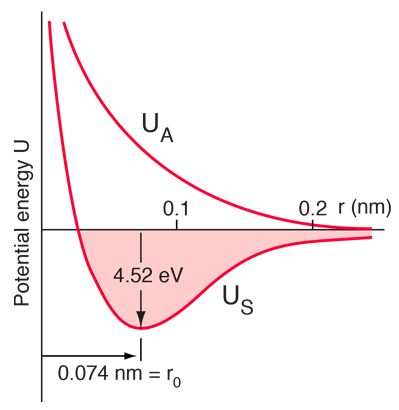
\includegraphics[width=0.3\textwidth]{./images/H2.png}
    \caption{Поверхность потенциальной энергии H\(_2\)}
    \label{fig:H2PPE}
\end{wrapfigure}
Поскольку ядра значительно тяжелее электронов, их движение происходит медленнее, чем у электронов. Поэтому хорошей аппроксимацией можно считать, что электроны в молекуле движутся в поле неподвижных ядер. 
Следовательно, в (\ref{eq:kin}) можно пренебречь вкладом \(\hat{T}_n\), а \(\hat{V}_{nn}\) можно считать константой, что не влияет на собственные функции гамильтониана, поэтому он приводится к виду
\begin{equation}
    \hat{H}_e = \hat{T}_e + \hat{V}_{ne} + \hat{V}_{ee} + V_{nn},
    \label{eq:H_e}
\end{equation}
Потенциал \(V_{nn}\) часто включают в гамильтониан, чтобы корректнее интерпретировать спектр с точки зрения физического смысла.
Таким образом приходим к электронному уравнению Шрёдингера

\begin{equation}
    \hat{H}_e \psi_e (\bm{r}| \bm{R} ) = E_e (\bm{R}) \psi_e (\bm{r}| \bm{R}),
    \label{eq:elH}
\end{equation}
где положение ядер \(\bm{R}\) является параметром.



Энергия \(E_e(\bm{R})\) может быть использована как потенциал при решении задачи движения ядер. Множество её значений в зависимости от координат называется \textit{поверхностью потенцильной энергии} Её график в случае молекулы H\(_2\) указан на рисунке \ref{fig:H2PPE}. Имеется всего лишь одна координата - расстояние между ядрами, причём нижняя кривая соответствует синглетному состоянию (\(S = 0\)), или основному состоянию для спектра электронного гамильтониана в каждой точке \(\bm{R}\), а верхняя - триплентному (\(S = 1\)). 

Стоит отметить, что хотя массы электронов и ядер отличаются на порядки (\(10^3 \div 10^5\)) имеются и случаи, когда пренебрегать такой разницей уже нельзя. Например, при исследовании лёгких веществ с помощью мюонов. Помимо этого, приближение Борна-Оппенгеймера часто предполагает большое расстояние между поверхностями потенциальной энергии, и в связи с этим приводит к невозможности системы переходить между ними. Такое, в частности, наблюдается в молекулах ретиналя, отвечающих за детектирования света клетками нашего глаза. В условиях адиабатичности они бы не могли менять конформацию.

\begin{figure}[h] %{l}{0.6\textwidth}
    \centering
    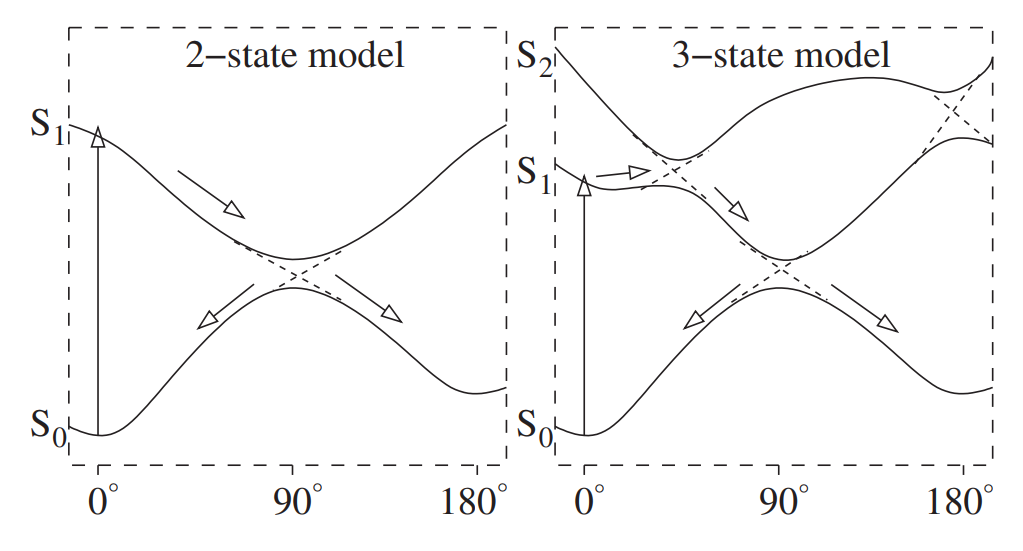
\includegraphics[width=0.6\textwidth]{./images/retinalePES.png}
    \caption{Поверхность потенциальной энергии ретиналя в двух наиболее распространённых моделях. \(0^{\circ}\) соответствует транс-конформации, \(180^{\circ}\) цис-конформации При поглощении фотона состояние системы переходит с ППЭ \(S_0\) на \(S_1\), где далее релаксирует до точки так называемого \textit{квазипересечения (avoided crossing)} или точки \textit{квазивырождения}, где учет неадиабатичности становится очень критичным, как читать может установить после прочтения данного параграфа.}
    \label{fig:retinalePES}
\end{figure}

\subsubsection*{Поправки в приближении Борна-Оппенгеймера}

Волновую функцию всей системы можно представить\footnote{При каждом фиксированном \(\bm{R}\) функция \(\psi(\bm{R})\) раскладывается по ортонормированному базису собственных функций электронного гамильтониана (\ref{eq:H_e}): \(\langle \psi_i | \psi_j \rangle = \delta_{ij}\).} как 

\begin{equation}
    \psi = \sum_{k=0}^{\infty} \chi_k (\bm{R}) \psi_k (\bm{r}| \bm{R})
\end{equation}
где \(\chi_k(\bm{R})\) - ядерные волновые функции


Тогда уравнение Шредингера \ref{eq:Shr} примет вид:
\begin{equation}
(\hat{T}_n + \hat{H}_e) \sum_k \chi_k (\bm{R}) \psi_k (\bm{r}| \bm{R}) = E \sum_k \chi_k (\bm{R}) \psi_k (\bm{r}| \bm{R})
\end{equation}

Домножим слева на \(\langle \psi_m|\):

\begin{equation}
\langle \psi_m | \hat{T}_n | \sum_k \chi_k \psi_k \rangle + \langle \psi_m | \hat{H}_e | \sum_k \chi_k \psi_k \rangle = E \langle \psi_m | \sum_k \chi_k \psi_k \rangle
\end{equation}

Воспользуемся ортонормированностью базиса: \(\langle \psi_m | \sum_k \chi_k \psi_k \rangle = \sum_k \chi_k \delta_{mk} = \chi_m\), а также тем, что \(\langle \psi_m | \hat{H}_e = \langle \psi_m | E_m \).

\begin{equation}
- \frac{1}{2} \sum_{k} \left[ \sum_\alpha \frac{1}{M_\alpha} \langle \psi_m |\nabla_\alpha^2 | \psi_k \chi_k \rangle \right]
+ E_m \chi_m = E \chi_m
\label{eq:shr1}
\end{equation}

Распишем лапласиан:

\[\nabla_\alpha \nabla_\alpha \chi_k \psi_k = \nabla_\alpha \left[(\nabla_\alpha \chi_k ) \psi_k + \chi_k (\nabla_\alpha \psi_k)\right] = (\nabla_\alpha^2 \chi_k ) \psi_k + 2 (\nabla_\alpha \chi_k) (\nabla_\alpha \psi_k ) + \chi_k (\nabla_\alpha^2 \psi_k)\]

Функция вида \((\nabla_\alpha \chi_k)\) зависит только от параметра \(\bm{R}\), поэтому её можно выносить из матричного элемента. В итоге слагаемое с суммой из (\ref{eq:shr1}) преобразуется так:

\begin{equation}
\begin{split}
    \sum_k \left(- \dfrac{1}{2} \sum_\alpha \dfrac{1}{M_\alpha} (\nabla_\alpha^2 \chi_k) \delta_{mk} - \sum_\alpha \dfrac{1}{M_\alpha} \langle \psi_m | \nabla_\alpha| \psi_k \rangle \nabla_\alpha \chi_k - \dfrac{1}{2} \sum_\alpha \dfrac{1}{M_\alpha} \langle \psi_m |(\nabla_\alpha^2 \psi_k) \rangle \chi_k \right) =\\
     = \underbrace{\left[- \dfrac{1}{2} \sum_\alpha \dfrac{1}{M_\alpha} \nabla_\alpha^2 \right]}_{\hat{T}_n} \chi_m - \sum_k \sum_\alpha \dfrac{1}{M_\alpha} \langle \psi_m | \nabla_\alpha | \psi_k \rangle \nabla_\alpha \chi_k - \dfrac{1}{2} \sum_k \sum_\alpha \dfrac{1}{M_\alpha} \langle \psi_m |(\nabla_\alpha^2 \psi_k) \rangle \chi_k 
\end{split}
\end{equation}

Таким образом (\ref{eq:shr1}) переходит в 

\begin{equation}
    \hat{T}_n \chi_m + E_m \chi_m - \sum_k \left[\sum_\alpha \dfrac{1}{M_\alpha} \overbrace{\langle \psi_m |\nabla_\alpha | \psi_k \rangle}^{A_{mk}} \nabla_\alpha \right] \chi_k - \dfrac{1}{2} \sum_k \left(\sum_\alpha \overbrace{\langle \psi_m | \nabla^2_\alpha | \psi_k \rangle}^{B_{mk}} \right) \chi_k = E \chi_m 
    \label{eq:shr2}
\end{equation}

Попробуем упростить данное уравнение. Рассмотрим при каких условиях можно пренебречь недиагональными матричными элементами.

Оценим \(A_{mk}\). При \(m = k\) в случае выбора вещественных волновых функций.

\[0 = \nabla_\alpha \langle \psi_m | \psi_m \rangle = 2 \langle \psi_m | \nabla_\alpha \psi_m \rangle\]

При \(m \neq k\)

\[0 = \nabla_\alpha \langle \psi_m | \hat{H}_e| \psi_k \rangle = E_k \langle \nabla_\alpha \psi_m | \psi_k \rangle + \langle \psi_m | (\nabla_\alpha \hat{H}_e) | \psi_k \rangle + E_m \langle \psi_m | \nabla_\alpha \psi_k \rangle \]

Откуда, пользуясь тем, что \(\langle \psi_m | \nabla_\alpha \psi_k \rangle = - \langle \nabla_\alpha \psi_m | \psi_m \rangle\), получаем

\begin{equation}
    A_{mk} = \langle \psi_m | \nabla_\alpha \psi_k \rangle = \dfrac{\langle \psi_m | (\nabla_\alpha \hat{H}_e )| \psi_k \rangle}{E_k - E_m}
    \label{eq:bf}
\end{equation}

Уравнение (\ref{eq:bf}) называется \textit{формулой Борна-Фока}. В случае, если \(A_{mk} \ll A_{mm}\), \(m \neq k\), что характерно для больших расстояний между энергиями \(E_k\) и \(E_m\), в уравнении (\ref{eq:shr2}) можно пренебречь слагаемыми с \(A_{mk}\), \(m \neq k\). Аналогично пренебрегаются и \(B_{mk}\), \(m \neq k\), как поправки второго порядка к неадиабатичности.

С учётом вышесказанных приближений уравнение (\ref{eq:shr2}) переходит в

\begin{equation}
    \left[ \hat{T}_n + E_m (\bm{R}) \right] \chi_m + \overbrace{\langle \psi_m | \hat{T}_n | \psi_m \rangle}^{B_{mm}} \chi_m = E \chi_m
    \label{eq:shr3}
\end{equation}

Матричный элемент \(B_{mm}\) называется диагональной Борн-Оппенгеймееровской поправкой (DBOS).
С DBOS уравнение (\ref{eq:shr3}) записано в \textit{адиабатическом приближении}. Без DBOS в \textit{приближении Борн-Оппенгеймера}:

\begin{equation}
    \left[ \hat{T}_n + E_m (\bm{R}) \right] \chi_m = E \chi_m
\end{equation}

\textbf{Задача.} Оцените поправку \(B_{mn}\) в приближении Борна-Оппенгеймера.

\subsection{Электронное уравнение Шрёдингера. Детерминанты слейтера}

Напомним вид уравнения Шрёдингера для системы электронов:

\[
\hat{H}_e \psi_e (\bm{r}| \bm{R} ) = E_e (\bm{R}) \psi_e (\bm{r}| \bm{R}), \tag{\ref{eq:elH}}
\]

Прежде, чем его решать, нужно потребовать некоторые условия на волновую функцию, а именно

\begin{enumerate}[label=\arabic*)]
\item \(\int |\psi_e|^2 d\bm{r}d\sigma = 1\)
\item \(\psi(\bm{r_1}, \bm{r_2}, \dots) = - \psi(\bm{r_2}, \bm{r_1}, \dots)\) (антисимметричность по перестановкам)

Асимптотические свойства:



\item \(\psi(\bm{r} \rightarrow \infty) \sim e ^{-r}\)
\item \(\psi(\bm{r} \rightarrow \bm{R}_\alpha) \sim e ^{- \alpha |r - R_\alpha|}\)
\item \(\psi(\bm{r}_1 \rightarrow \bm{r_2}) \sim \alpha |r_1 - r_2| + C\)
\end{enumerate}

Последнее свойство является самой тяжелой преградой для численного решения электронного уравнения Шрёдингера. То есть у функции при стремлении позиций электронов друг к другу должен быть излом и потеря гладкости.

Теперь воспользуемся методом Фурье для решения \eqref{eq:elH}. Для этого представим решение в виде

\begin{equation}
    \psi_e = \sum_k c_k \Phi_k,
\end{equation}
где базисные функции \(\Phi_k\) являются многоэлектронными и является антисимметричными по перестановкам. Помимо этого \(\langle \Phi_k | \Phi_l \rangle = \delta_{kl}\).

Рассмотрим в качестве примера систему из двух электронов (атом гелия)

Наивная попытка оставить волновую функцию будет следующей:

\begin{equation}
    \psi_e = \phi_{1s}(\bm{r}_1) \phi_{1s}(\bm{r}_2),
    \label{eq:psi_e_naive}
\end{equation}
однако такая функция не удовлетворяет запрету Паули и не учитывает спин.

Введём следующие обозначения:

\begin{equation}
    \eta = \alpha = \begin{pmatrix} 1 \\ 0 \end{pmatrix}, \;
    \eta = \beta = \begin{pmatrix} 0 \\ 1 \end{pmatrix}
\end{equation}

Переменная \(\alpha\) соответствует состоянию спина вверх, а \(\beta\) — вниз. С помощью скобок \(\alpha(i)\) будем обозначать состояние спина \(i\)-го электрона. Например, \(\alpha(1)\) означает, что первый электрон имеет спин вверх. 

Теперь, чтобы создать правильную многоэлектронную волновую функцию вместо \eqref{eq:psi_e_naive} антисимметризуем её (\(\psi_{antisym} = \psi(\bm{r}_1, \bm{r}_2) - \psi(\bm{r}_2, \bm{r}_1)\)) и добавим спин:

\begin{multline}
\psi_e = \psi_{1s} (\bm{r}_1) \psi_{1s} (\bm{r}_2) = \frac{1}{\sqrt{2}} \phi_{1s} (\bm{r_1}) \alpha(1) \phi_{1s} (\bm{r}_2) \beta(2) - \frac{1}{\sqrt{2}} \phi_{1s} (\bm{r_2}) \alpha(2) \phi_{1s} (\bm{r}_1) \beta(1) =\\=
\begin{vmatrix}
\phi_{1s} (\bm{r_1}) \alpha(1) & \phi_{1s} (\bm{r_2}) \alpha(2) \\
\phi_{1s} (\bm{r_2}) \beta(1) & \phi_{1s} (\bm{r_1}) \beta(2)
\end{vmatrix}
\end{multline}

В общем случае, вспомнив формулу для определителя, детерминант Слейтера можно записать так:

\begin{equation}
    \Phi_e = \dfrac{1}{\sqrt{N!}} \sum_{K = \sigma(k_1, \dots, k_N)} (-1)^p \psi_{k_1} (1) \dots \psi_{k_N} (N)
\end{equation}

Большинство задач требуют расчёта матричного элемента:
\begin{equation}
    \langle \psi_e | \hat{A} | \psi_e \rangle,
\end{equation}
где \(\hat{A}\) - произвольный оператор. Это приводит задачу к тому, что нужно считать матричные элементы по детерминантам Слейтера:

\begin{equation}
\langle \psi_e | \hat{A} | \psi_e \rangle = \sum_{K, L} c_K^* c_L \langle \Phi_K | \hat{A} | \Phi_L \rangle,
\end{equation}
чего мы пока что делать не умеем. Напрямую считать это невозможно, поскольку, например, при \(N = 100\) (вообще говоря типичное значение для молекул), и соответственно \(N!\) мы никак не посчитаем, поэтому нужно придумать определённые правила для расчёта данных матричных элементов.

Для того, чтобы задать детерминант слейтера, нужно иметь одноэлектронные волновые функции. Чтобы ими воспользоваться рассмотрим следующую модель: рис. \ref{fig:spinorbitals}. Положим, что в нашей системе \(N\) электронов, \(M\) спин-орбиталей, и \(M \gg N\).

\begin{figure}
    \centering
    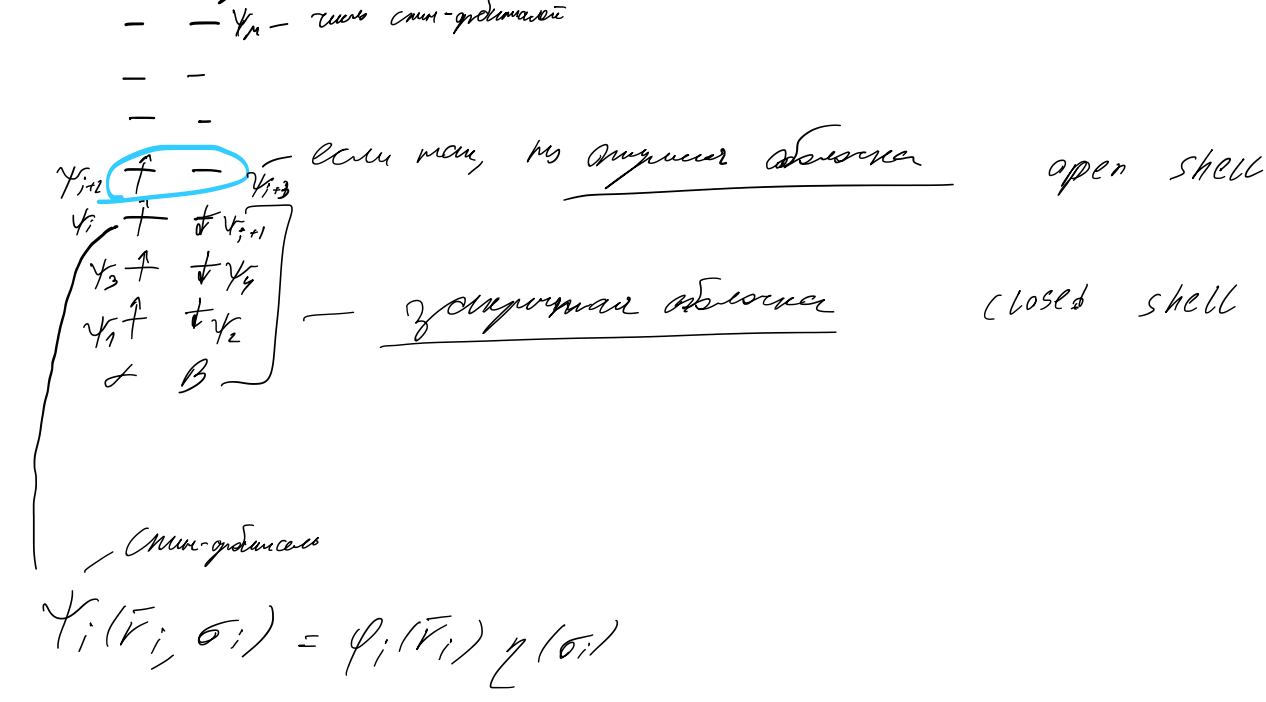
\includegraphics[width=0.7\textwidth]{./images/spin-orbitals.png}
    \caption{Электронная конфигурация}
    \label{fig:spinorbitals}
\end{figure}

Детерминант слейтера, соответствующий основной конфигурации можно записать следующим образом: 

\begin{equation}
\Phi_0 = const \sum_{K = \sigma(i_1, \dots i_N)} (-1)^{P(K)} \psi_{i_1}(1) \dots \psi_{i_N}(N)
\end{equation}
Потребуем следующее: \(\langle \Phi_0 | \Phi_0 \rangle = 1\)

\begin{multline}
1 = |const|^2 \left\langle \sum_{K = \sigma(i_1, \dots, i_N)} (-1)^{P(K)} \psi_{i_1} (1) \dots \psi_{i_N} (N) \middle| \sum_{L = \sigma(j_1, \dots, j_N)} (-1)^{P(L)} \psi_{j_1} (1) \dots \psi_{j_N} (N) \right\rangle =\\= 
|const|^2 \sum_{K = \sigma(i_1, \dots, i_N)} (-1)^{P(K)} \sum_{L = \sigma(j_1, \dots, j_N)} (-1)^{P(L)} \underbrace{\langle \psi_{i_1} (1) \dots \psi_{i_N} (N) | \psi_{j_1} (1) \dots \psi_{j_N} (N) \rangle}_{\langle\psi_{i_1} (1) | \psi_{j_1} (1) \rangle \dots \langle \psi_{i_N(N)} | \psi_{j_N}(N) \rangle},
\label{eq:phi00}
\end{multline}
где в последнем бракет мы разделили интеграл по отдельным переменным. Теперь давайте потребуем ортогональность спин-орбиталей \(\langle \psi_i | \psi_j \rangle = \delta_{ij}\) (однако существуют и случаи, когда некоторые обходятся и без этого предположения, что может быть, например, в системах нейтральной молекула + катион). Таким образом \eqref{eq:phi00} сводится к:
\begin{multline}
1 = |const|^2 \sum_{K = \sigma(i_1, \dots, i_N)} (-1)^{P(K)} \sum_{L = \sigma(j_1, \dots, j_N)} (-1)^{P(L)} \delta_{i_1 j_1} \dots \delta_{i_N j_N} =\\=
|const|^2 \sum_{K = \sigma (i_1, \dots, i_N)} 1 = N! \; |const|^2 = 1,
\label{eq:phiphi}
\end{multline}
\begin{wrapfigure}{r}{0.2\textwidth}
    \centering
    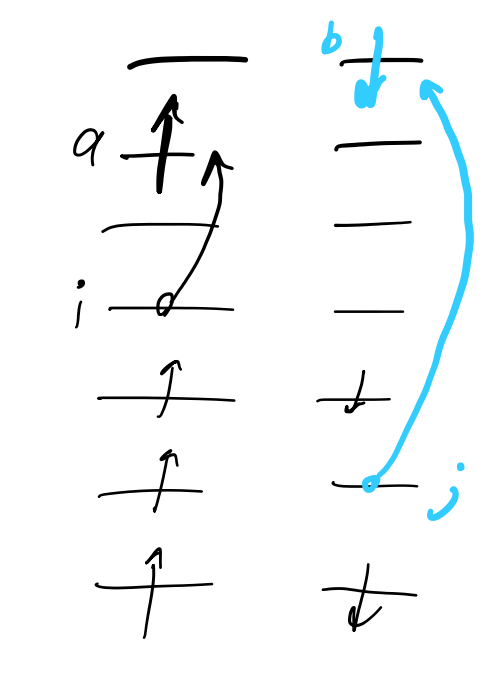
\includegraphics[width=0.2\textwidth]{./images/spin-orbitals3.png}
    % \caption{Возбуждённые состояния}
    % \label{fig:spin-orbitals3}
\end{wrapfigure}
откуда получаем значение нормировочной константы: \(const = \dfrac{1}{\sqrt{N!}}\)

Как теперь сгенерировать детерминанты помимо \(\Phi_0\)? Для этого введём следующие обозначения: рис. \ref{fig:spin-orbitals2}. Будем обозначать детерминанты возбуждённых состояний следующим образом:
\begin{equation}
\Phi_i^a = \hat{a}_a^\dag \hat{a}_i \Phi_0,
\end{equation}
где \(\hat{a}_a^\dag \hat{a}_i\) -- оператор однократного возбуждения. Аналогично можно задавать и двакратно возбуждённые состояния:
\begin{equation}
\Phi_{ij}^{ab} = \hat{a}_a^\dag \hat{a}_i \hat{a}_b^\dag \hat{a}_j \Phi_0.
\end{equation}

Обычно операторы записывают в порядке \(i < j, a < b\). Обозначим \(M - N = N_{virt}\), \(N = N_{occ}\), тогда число возможных однократно возбуждённых состояний: \(N_{virt} \cdot N_{occ}\), а двукратно возбуждённых:

\[
\frac{N_{virt}(N_{virt} - 1)}{2} \cdot \frac{N_{occ}(N_{occ} - 1)}{2}
\]

\begin{figure}
    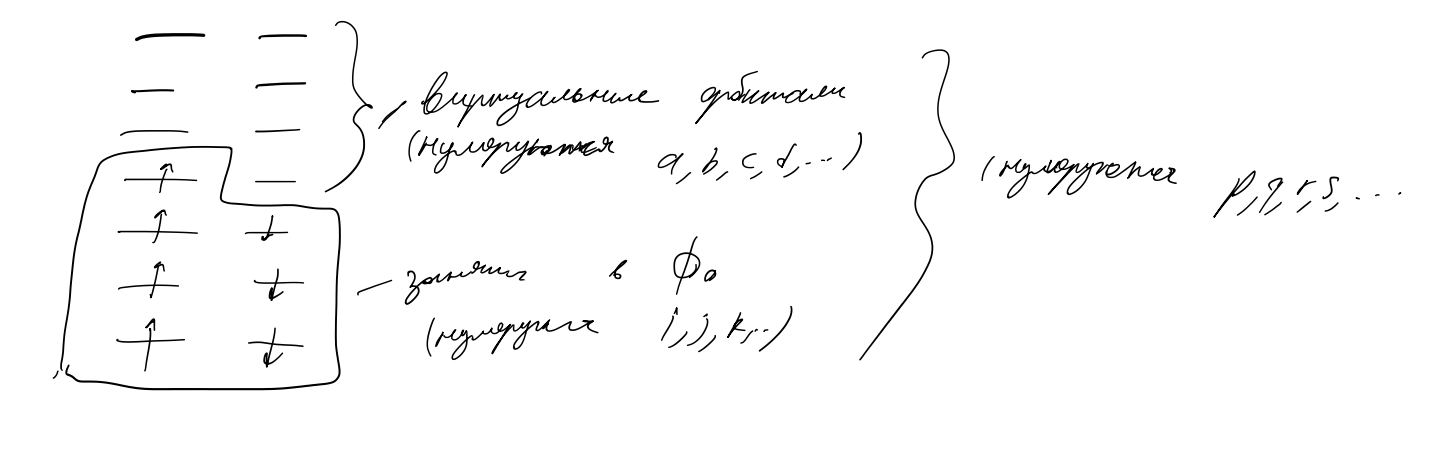
\includegraphics[width=0.7\textwidth]{./images/spin-orbitals2.png}
    \caption{Обозначения для спин-орбиталей}
    \label{fig:spin-orbitals2}
\end{figure}

Часто задачи требуют двукратно и трёхкратно вырожденные состояния, но это уже для некоторых молекул, как нетрудно заметить, довольно большой базис. 


Нетрудно проверить ортогональность произвольных детерминантов Слэйтера при \(K \neq L\):

\[\langle \Phi_K | \Phi_L \rangle = 0,\]
поскольку в сумме, аналогичной \eqref{eq:phiphi} обязательно возникнет дельта-символ \(\delta_{i_{p}j_{q}} = 0\), где \(\psi_q\) и \(\psi_q\) - разные орбитали.

Теперь вычислим научимся вычислять матричные элементы операторов:

\begin{equation}
\hat{a}(i) = \sum_{i=1}^{N} \left(- \dfrac{1}{2} \nabla_i^2 - \sum_\alpha \dfrac{Z_\alpha}{|\bm{R}_\alpha - \bm{r}_i|}\right), \hat{b}(i, j) = \dfrac{1}{2} \sum_{i\neq j } \dfrac{1}{|\bm{r}_i - \bm{r}_j|},
\end{equation}
где \(\hat{a}(i)\) - одноэлектронная часть гамильтониана, а \(\hat{b}(i, j)\) - двухэлектронная часть гамильтониана. Дальнейшие выводы будут верны и для любых других одноэлектронных или двухэлектронных операторов.

Начнём с диагонального элемента \(\langle \Phi_0 | \hat{a}(i) | \Phi_0 \rangle\):

\begin{multline}
\langle \Phi_0 | \hat{a}(i) |\Phi_0 \rangle =\\= \dfrac{1}{N!} \sum_{K = \sigma(i_1, \dots i_N)} \sum_{L = \sigma(j_1, \dots j_N)} (-1)^{P(K)} (-1) ^ {P(L)} \sum_p \langle \psi_{i_1} (1) \dots \psi_{i_N} (N) | \hat{a} (p) | \psi_{j_1} \dots \psi_{j_N} (N) \rangle =\\=
 \dfrac{1}{N!} \sum_{K} \sum_{L} (-1) ^{P(K)} (-1) ^ {P(L)} \sum_p \langle \psi_{i_p} | \hat{a} (p) | \psi_{i_p} (p) \rangle \delta_{i_1 j_1} \dots \delta_{i_N j_N} =\\=
\dfrac{1}{N!} \sum_{K = \sigma(i_1, \dots i_N)} \sum_p \langle \psi_{p} (p) | \hat{a} (p) | \psi_{p} (p) \rangle = \sum_p \langle \psi_{p}(1) | \hat{a}(1) | \psi_{p}(1) \rangle
\end{multline}
Обратите внимание, что в последнем равенстве мы перешли от интегрирования по каждому из электронов к интегрированию по одному, но по разным орбитальным функциям.

\textbf{Задача.} Покажите, что

\[\langle \Phi_0 | \sum_p \hat{a} (p) | \Phi_i^a \rangle = \langle \psi_i (1) | \hat{a}(1) | \psi_a (1) \rangle\]

\[\langle \Phi_0 | \sum_p \hat{a} (p) | \Phi_{ij}^{ab} \rangle = 0\]

Теперь перейдём к двухэлектронному оператору.

\begin{multline}
\langle \Phi_0 | \sum_{p\neq q}\hat{b}(i, j) | \Phi_0 \rangle =\\= \dfrac{1}{N!} \sum_{K = \sigma(i_1, \dots i_N)} \sum_{L = \sigma(j_1, \dots j_N)} (-1)^{P(K)} (-1) ^ {P(L)} \sum_{p, q} \langle \psi_{i_1} (1) \dots \psi_{i_N} (N) | \hat{b} (p, q) | \psi_{j_1} \dots \psi_{j_N} (N) \rangle,
\end{multline}
нас будут интересовать только матричные элементы вида \(\langle \psi_{i_p} (p) \psi_{i_q} (q) | \hat{b} (p, q) | \psi_{j_p} (p) \psi_{j_q} (q) \rangle\), поскольку слагаемые содержащие \(\langle \psi_{i_p}(p) \psi_{i_r} (q) | \hat{b} | \psi_{j_p}(p), \psi_{j_q}(q) \rangle, r \neq p, q\) будут равны нулю из-за наличия множителя \(\langle \psi_q(q) | \psi_r (q) \rangle = 0\). При перестановке двух орбиталей четность перестановки меняется и таким образом:

\begin{equation}
\langle \psi_{i_p} (p) \psi_{i_q} (q) | \hat{b} (p, q) | \psi_{j_p} (p) \psi_{j_q} (q) \rangle = - \langle \psi_{i_p} (p) \psi_{i_q} (q) | \hat{b} (p, q) | \psi_{j_q} (p) \psi_{j_p} (q) \rangle
\end{equation}
Таких слагаемых будет по два с учётом того, что сопряженные матричные элементы равны друг другу. В результате оставшихся дельта-символов сумма по одной из перестановок уходит, и при этом остается \(N - 2\) независимых индексов, по которым можно проводить оставшуюся перестановку. То есть вместо числа перестановок \(N!\) как в прошлый раз, мы будем иметь \(A_{N}^{N-2}\) (количество способов выбрать \(N-2\) элементов из \(N\)), что равно \(N (N-1) (N-2) \cdot ... \cdot 3 \). Не забывая о коэффициенте \(\frac{1}{N!}\) получаем итоговый ответ:

\begin{multline}
\langle \Phi_0 | \dfrac{1}{2} \sum_{p \neq q} \hat{b}(p, q) | \Phi_0 \rangle =\\=
\frac{1}{2} \sum_{p\neq q} 
\left[\langle \psi_p(1) \psi_q (2) |\hat{b} (1, 2)| \psi_p (1) \psi_q (2) \rangle  - \langle \psi_p(1) \psi_q (2) | \hat{b} (1, 2) | \psi_q (1) \psi_p (2) \rangle \right],
\label{eq:doublemat}
\end{multline}
где вклад от первого слагаемого называют кулоновским, а от второго обменным. 

Давайте несколько упростим обозначения: перестанем писать букву \(\psi\),номера электронов и введём обозначение антисимметризации \(||\). Тогда \eqref{eq:doublemat} упрощается следующим образом:

\begin{equation}
\langle \Phi_0 | \dfrac{1}{2} \sum_{p \neq q} \hat{b}(p, q) | \Phi_0 \rangle =
\dfrac{1}{2}\sum_{p, q} \langle p q || p q \rangle
\end{equation}

\textbf{Задача.} Проверьте, что 

\[\langle \Phi_0 | \dfrac{1}{2} \sum_{p \neq q} \hat{b}(p, q) | \Phi_i^a \rangle = \sum_{p} \langle p i || p a \rangle\]

\[\langle \Phi_0 | \dfrac{1}{2} \sum_{p \neq q} | \Phi_{ij} ^{a b} \rangle = \langle i j  || a b \rangle\]

\[\langle \Phi_0 | \dfrac{1}{2} \sum_{p \neq q} | \Phi_{ijk} ^{a b c} \rangle = 0\]

Может возникнуть вопрос, почему произошёл выбор именно в пользу такой модели спин-орбиталей и детерминантов. Дело в том, что на практике часто сами детерминанты считать не нужно, нужны только спин орбитали, поэтому детерминанты часто хранят в виде \(\Phi = [1 1 1 1 0 1 0 0 0 0 \dots]\) и операции по вычислению матричных элементов становятся тривиальными, как например, побитовое умножение. Такая простота позволяла ещё на раннем этапе вычислительной техники сильно зарекомендовать данную модель как лидера, которым она остается благодаря этой простоте и по сей день.

\subsection{Спин-орбитали}

Мы до этого момента воспринимали наличие спин-орбиталей как данность. Разберёмся, откуда их можно получить. Прежде, чем перейти к этом разберёмся в том, нужны ли нам все детерминанты Слейтера, можно ли пренебречь как-либо частью базисных элементов? Как мы помним

\[\psi_e = \sum_K c_K \Phi_K,\]
причём можно выделить два случая:

\begin{multicols}{2}
\subsubsection*{Одноконфигурационная волновая функция. Single-reference (SR)}

\[C_0 \Phi_0 + \sum_{L > 0} C_L \Phi_L\]

Характерно для замкнутых оболочек высокоспиновых состояний. Как правило, основное состояние с равновесной геометрией. Разрывы связей сюда не входят.

\columnbreak

\subsubsection*{Многодетерминантная волновая функция. Multi-reference (MR)}
\[\sum_\mu C_\mu \Phi_\mu + \sum_{L > N_\mu } c_L \Phi_L\] 


Первая часть слагаемых называется модельными детерминантами и отвечает за качественное описание системы. 

\(span\{\Phi_\mu\}\) - модельное пространство

Характерно для открытых оболочек, возбужденных состояний, переходных металлов. Описывает разрывы связей.
\end{multicols}

Мы будем в дальнейшем заниматься в основном single-reference системами.

{\color{red}Теперь вернёмся к задаче поиска спин-орбиталей. Будем их вычислять также в одноконфигурационных системах. Будем исходить из последовательных приближений:

\[\psi_e = \Phi_0 + \cancel{\dots}\]

Если выбрать в качестве волновой функции один детерминант Слэйтера, то мы получим:

\[\psi_e = \Phi_0,\]
что по сути представляет собой метод Хартри-Фока, или же метод самосогласованного поля, откуда мы получаем набор \(\{\psi_p\}\)

Если \(\psi_e = \varepsilon c_\mu \Phi_\mu + \cancel{\dots},\)
то метод будет называться многоконфигурационным методом самосогласованного поля.}\footnote{Поправить, пропустил лекцию}

Посчитаем \(\langle \psi_e | \hat{H}_e | \psi_e \rangle \approx \langle \Phi_0 | \hat{H}_e | \Phi_0 \rangle\). Как известно из квантовой механики, это даст оценку сверху на значение минимальной энергии в спектре. Далее воспользовавшись методом поиска основного состояния в классе пробных функций, мы сделаем более точную оценку, минимизировав данную энергию в зависимости от спин-орбиталей (вариационный принцип). Вспомнив одноэлектронную часть гамильтониана:

\begin{equation}
\hat{h} = \sum_{i=1}^{N} \left(- \dfrac{1}{2} \nabla_i^2 - \sum_\alpha \dfrac{Z_\alpha}{|R_\alpha - r_i|}\right)
\end{equation}
и двухэлектронную:
\begin{equation}
\hat{g} = \dfrac{1}{2} \sum_{i \neq j} \dfrac{1}{|\bm{r}_i - \bm{r}_j|},
\end{equation}
выбросив константу и воспользовавшись правилами Слейтера, мы получаем следующий ответ:
\begin{equation}
E_e = \sum_{i=1}^N \langle \psi_i | h | \psi_i \rangle + \dfrac{1}{2} \sum_{i \neq j} \langle ij || ij \rangle .
\end{equation}
Далее нам нужно найти при каких \(\psi_i\) данный функционал \(E[\psi_i]\) достигает минимума при условии \(\langle \psi_i | \psi_j \rangle \)

\end{document}
